\documentclass[12pt]{article}

% Packages
\usepackage[english]{babel}
\usepackage[hyphens]{url}
\usepackage{hyperref}
\usepackage[citestyle=authoryear, bibstyle=authoryear, sorting=nyt]{biblatex}
\usepackage{breakurl}
\usepackage{caption} % for customizing captions
\usepackage[autostyle, english = american]{csquotes}
\usepackage{dot2texi}
\usepackage{etoolbox} % for adjusting environment parameters
\usepackage{fancyhdr} % for custom headers and footers
%\usepackage{fontspec} % for setting fonts
\usepackage[margin=1in]{geometry} % for setting margins
\usepackage{graphicx} % for including graphics
\usepackage{parskip} % for controlling paragraph spacing
%\usepackage{pxfonts}
\usepackage{setspace} % for adjusting line spacing
\usepackage{tikz}
\usepackage{titlesec} % for customizing section headings
\usepackage{breakurl}
\def\UrlBreaks{\do\/\do-}

\addbibresource{1_SOC_Honors.bib} % Replace with your .bib file

\MakeOuterQuote{"}

% Line spacing
\setstretch{2}

% Paragraph spacing
\setlength{\parskip}{0pt}

% Define indentation length
\newlength{\myindent}
\setlength{\myindent}{3em}

% Set the hanging indent
\setlength{\bibhang}{\myindent}

% Redefine the citation command to use colon instead of comma and pp.
\DeclareFieldFormat{postnote}{#1}
\DeclareFieldFormat{multipostnote}{#1}

% Use colon (ASA Style) in-text citations (author year:page)
\renewcommand*{\postnotedelim}{\addcolon}

% Set global text alignment to ragged-right
\raggedright

% Paragraph indentation
\setlength{\parindent}{\myindent}

% Font
% \setmainfont{Times New Roman}

% Define a variable for the title
\newcommand{\myTitle}{CONSTRUCTION UNIONS HISTORICAL-COMPARATIVE}

\newcommand{\imageWidth}{0.8\textwidth}

% Page style
\pagestyle{fancy}
\fancyhf{} % clear all header and footer fields
\fancyhead[R]{\thepage} % page number on the right side
\fancyhead[L]{\small \myTitle}
\renewcommand{\headrulewidth}{0pt} % remove header rule

% Customize abstract page
\renewenvironment{abstract}
  {\par\noindent\centering\textbf{Abstract}\par\noindent\raggedright}
  {\par}

% Redefine the quote environment
\renewenvironment{quote}
  {\list{}{\leftmargin=\parindent\rightmargin=0pt}%
   \item\relax}
  {\endlist}
  
% Redefine the quote environment to make it single-spaced and remove vertical space before and add one at the end
\AtBeginEnvironment{quote}{\singlespacing\setlength{\topsep}{0pt}\setlength{\partopsep}{0pt}}
\AtEndEnvironment{quote}{\vspace{0.5\baselineskip}}

\begin{document}

\begin{titlepage}
  \thispagestyle{fancy}
  \pagenumbering{gobble}
  \fancyhead[L]{Running head: \myTitle}
  \centering
  \vspace*{1.95in}
  {\LARGE Construction Union Agreements:\par Union Organizing in Historical-Comparative Perspective\par}
  \vspace{1.2in}
  {Matthew A. Carson\par}
  \vspace{0in}
  {University of California, Los Angeles\par}
  \vspace{0.5in}
  {\today\par}
%  \vfill
%  \wordcount
\end{titlepage}

% Set page numbering to roman for preliminary pages
\pagenumbering{roman}

% Add abstract page
\begin{abstract}
US Building Trade unions organize their workers differently. Most labor unions compel employers to negotiate, but the Building Trades engage in voluntary negotiations, relying on workers' skill levels rather than strike leverage. This approach correlates with their frequent political deviations from the broader US labor movement, particularly in opposing progressive environmental policies and aligning more closely with the petrochemical industry on environmental issues, and not supporting single-payer healthcare. One view is that unions pursue their members’ interests narrowly, sacrificing broader working-class interests if they feel it is necessary to secure work for their members, and some suggest that the conservative stance of the Building Trades stems from their craft union tradition, in which workers are organized by craft and skill instead of by industry. However, using historical-comparative methods, I show that these arguments do not hold. Petrochemical unions have supported progressive policies, and other craft-based unions have endorsed single-payer healthcare. However, unlike the Building Trades, those unions have never used voluntary agreements. Consequently, they have experienced more conflicts with employers. These findings challenge traditional views and suggest that the Building Trades' conservative negotiation strategies significantly shape their political and policy positions, reinforcing an employer-union dynamic that limits challenging management.
\end{abstract}
\newpage

% Add table of contentsart
\tableofcontents
\newpage

\listoffigures
\newpage

% Define custom section headings
\titleformat{\section}[block]{\normalfont\fontsize{12}{14}\selectfont\bfseries}{\thesection.}{0.5em}{}
\titleformat{\subsection}[block]{\itshape\bfseries}{\thesubsection.}{0.5em}{}
\titleformat{\subsubsection}[runin]{\normalfont\itshape\bfseries}{\hspace{\myindent}\thesubsubsection.}{0.5em}{}[.]

% Set page numbering to arabic for main content
\pagenumbering{arabic}

%\section{INTRODUCTION} \
\addcontentsline{toc}{section}{Introduction}

Construction is one of the largest unionized sectors in the United States. In spite of this, labor research has largely not focused on construction unions (or what are often referred to as the Building Trades) but has focused mainly on how workers in other industries organize. In some sense, this is understandable. One of the most significant periods of union growth in the US was in the 1930s, when multiple violent strikes occurred, sometimes lasting for a month or longer. These events contributed to the rise of the Congress of Industrial Unionism (CIO), a federation of trade unions committed to industrial unionism rather than craft unionism. Congress and President Franklin D. Roosevelt responded to these violent battles by enacting the Wager Act, which guaranteed the right for workers to organize and provided a framework for workers to petition for union representation in the workplace (\cite{grossMakingNationalLabor1974}). This framework was adapted mainly to how industrial unions were organized at the time. Most unionization efforts, especially large-scale and prominent ones, have used the industrial union organizing model.

% Add a citation for month-long strikes and how they led to the Wagner Act.
% Gross, James A. 1974. The Making of the National Labor Relations Board: A Study in Economics, Politics, and the Law. Albany: State University of New York Press.

US construction unions have a distinct approach to organizing their workers vis-à-vis other labor unions. While most labor unions typically compel employers to negotiate through secret ballot elections or work stoppages, the Building Trades take a different route by engaging in voluntary negotiations. Their strategy hinges more on the skill levels of their workers than the leverage of strikes or official National Labor Relations Board elections, which use the state to compel the employer to negotiate. This unique approach often leads them to deviate politically from the broader US labor movement. Notably, they frequently oppose progressive environmental policies and tend to align more closely with the petrochemical industry on environmental issues. Additionally, they are not supportive of single-payer healthcare.

One potential explanation is that unions with many workers in the petrochemical industry will align with the employer on environmental policy if they feel that environmental policies might be "job killers." That is, the Building Trades' opposition to environmental policy meant to attenuate global warming might simply be a function of the union's interest in keeping their members working. They have many members working on projects in the petrochemical industry, and this is what one would expect from workers and their unions in that industry. After all, why would they support something that might cause unemployment?

Some argue that the conservative stance of the Building Trades originates from their tradition of craft unionism, where workers are organized based on craft and skill rather than industry. Craft unions were some of the earliest labor organizations in the US. And their focus on organizing narrowly based on craft distinctions (e.g., plumber) rather than by industry (e.g., construction worker) often corresponded with nativist and racist policies and positions and more conservative positions (e.g., anti-communism and redbaiting) than many industrial unions (\cite{foner1994}). In short, they have tended to look out for "their own" more so than workers more broadly. The Building Trades unions continue to operate as craft unions today.\footnote{You can find a union for almost every construction craft --- electricians, plumbers, bricklayers, and so on --- but good luck finding a union called the "Construction Workers Union."} From this perspective, the Building Trades' conservativism stems from their narrow craft-based unionism.

However, these views are mistaken. For instance, other unions with many members working in the petrochemical industry, such as the United Steelworkers, have backed progressive policies, including environmental policies, and other craft-based unions, such as the International Association of Machinists, have endorsed single-payer healthcare despite organizing along craft lines instead of industry. The key distinction between these unions and their disparate political stances lies in the Building Trades' use of voluntary agreements, which minimizes conflicts with employers and constrains their ability to challenge management.

% Foner, Phillip S. History of the Labor Movement in the United States: Volume 2: From the Founding of the AFL to the Emergence of American Imperialism. New York: International Publishers, 1955; pp. 132–133.

\section{METHODS} \

I primarily use historical and comparative methods to analyze the inter-union (Building Trades vs. non-building Trades) cases. Following Lange (\citeyear{lange2013}), I employ both within-case and between-case (comparative) methods. This paper's within-case analyses are of the individual unions and their historical trajectories. This is the ideographic or historical element of the analysis. I trace each union's history and how institutions formed within the unions (e.g., the apprenticeship and hiring hall). This offers a thick account of how the unions have evolved, challenged management at points, fought for or against policies, and made compromises at times. It also pays close attention to each moment's context to prevent a linear, teleological account of history that suggests that the present state was inevitable because of something that happened in the past. I draw primarily from secondary sources for these historical accounts. Additionally, I interviewed a former Oil Chemical and Atomic Workers union member and official to supplement the historical account and gather more recent data about the current state of affairs of the union.\footnote{Now part of the United Steelworkers}

The comparison or between-case analysis focuses both on the differences in features of the union and on the differences in their historical trajectory. Each case either uses or does not use a voluntary/involuntary contract type. In one case, construction unions (craft unions) are compared against non-construction craft unions; in another, construction unions, which have a lot of members working in the petrochemical industry, are compared with a non-construction union also with a lot of members working in the petrochemical field. 

The intra-building trades analysis data were collected from interviews with local union officials. These local unions were located via the National Labor Relations Board case search tool. Each of these locals was involved in an organizing campaign that used the method that non-construction unions typically use (and construction unions typically do \textit{not} use). These cases where the construction union departed from the norm were compared against the more general trends in the building trades unions.

\section{CRAFT UNIONISM VS. INDUSTRIAL UNIONISM} \

Craft unionism is when workers are organized into a union by craft (occupation) rather than industry (or employer). The earliest efforts in the US to organize workers collectively to assert their interests and preferences were generally organized around craft lines. Plumbers formed their union; machinists started one; so did the carpenters, and so on. Many of these early craft unions were successful. Eventually, The American Federation of Labor (AFL) formed in 1886, bringing many of these labor unions into a nationwide federation. Immediately, many constituent unions battled over craft jurisdiction. For example, who should operate the mobile concrete mixers on the job site? Both the Teamsters and Operating Engineers claimed the work to be theirs at one point, leading to a jurisdictional dispute. As a result, one of the most important functions of the newly formed federation was to quell these jurisdictional fights (\cite{jaffe1940}).

% Jaffe, Louis L. 1940. “Inter-Union Disputes in Search of a Forum.” The Yale Law Journal 49(3):424–60. doi: 10.2307/792665.

Industrial unionism did not emerge until some time later. Industrial unionism organizes workers by employer or industry, irrespective of their craft, occupation, or skill level. Many early craft unionists in the AFL were skeptical of industrial unionism because many workers in mass-production factories were immigrants with no specific craft or formal training. AFL craft union leaders doubted the feasibility of organizing them, as these workers lacked the leverage typically associated with having a craft. Their jobs were often repetitive and required little skill. For instance, performing tasks like standing in one place and fastening bolts on a Model T all day did not constitute a craft, unlike the specialized skills of a machinist operating a lathe or a pile driver constructing a bridge.

\subsection{The Industrial Bargaining Approach}

The National Labor Relations Act was originally designed to be consistent with how industrial unions are organized. The National Labor Relations Act (NLRA) sets forth the process workers must follow to unionize a workplace. The National Labor Relations Board (NLRB) administers the NLRA. The typical process begins with an effort to determine if there is a general interest in forming or joining a union among workers already hired. If there appears to be enough interest, "employee organizers typically collect union interest cards, petitions or other written statements from co-workers to show interest in union representation. Organizing efforts may be supported by an established union seeking to represent workers at a workplace. Workers may also form an independent union" (\cite["How can I form a union?"]{dolWORKCenterUnions}). If enough cards are collected to demonstrate majority status, the workers may ask the employer to voluntarily\footnote{This is distinct from the voluntary negotiations in construction unionism. In this case, the employer may voluntarily recognize the union because they are certain that the majority of the workers want the union in the workplace, and conducting an election would be futile. In practice, this rarely happens, though.}  recognize the union. If the employer refuses to voluntarily recognize the union, workers may strike and/or file a petition with the NLRB to request an election to certify the union and the collective bargaining representative of the workers (\cite["How can I form a union?"]{dolWORKCenterUnions}; \cite{NLRBProcessNational}). Once the union has demonstrated that the majority of workers want union representation (either through voluntary recognition by the employer or through an NLRB election), the union and employer will attempt to reach an initial agreement (Figure \ref{fig:DOL}). This type of agreement is called a Section 9(a) agreement.

\begin{figure}[ht]
  \centering
  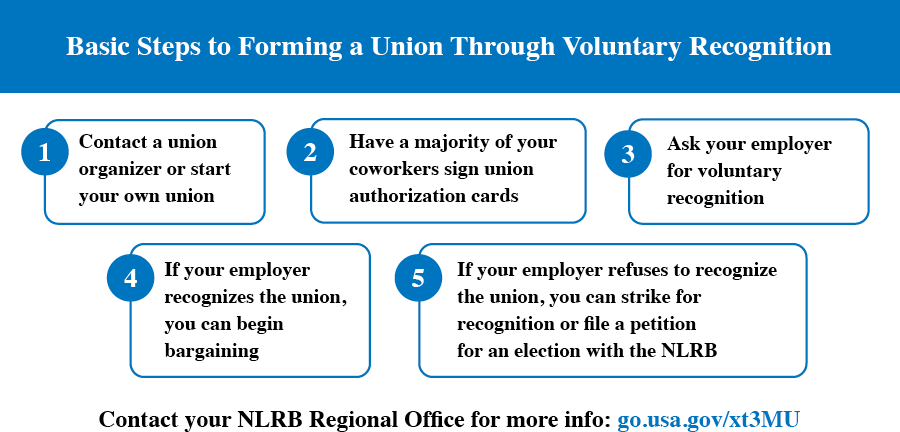
\includegraphics[width=\imageWidth]{images/DOL}
  \captionsetup{justification=centering, singlelinecheck=false, margin=2cm}
  \caption[Forming a Union]{The steps for forming a union or joining an existing union. (Source: US Department of Labor.)}
  \label{fig:DOL}
\end{figure}

If the employer refuses to negotiate, the union can file an "unfair labor practice." They can also strike or conduct other work stoppages until the recalcitrant employer meets their demands or agrees to negotiate. These are \textit{coercive} strategies that are meant to compel the employer to act or not act in a particular way or to exact concessions. These strategies are also \textit{more conflictual} relative to the Building Trades' approach.

\subsection{The Building Trades Approach}

In contrast to this approach, building and construction trade unions do not usually organize the workers at the workplace. They typically establish voluntary agreements with employers, which can be established before the employer hires any employees. Since these agreements can be established before any workers are hired, they are called prehire agreements. Prehire agreements have a long history that predates their legitimation by Congress in 1959 with the passage of the Labor-Management Reporting and Disclosure Act (LMRDA). In fact, before the LMRDA, the NLRB had refused to take jurisdiction over the building and construction trades because their approach to union organizing was so different, and in fact, would be an unfair labor practice, a violation of the NLRA, if they were to take jurisdiction over the matter. So, whereas labor law is often discussed in terms of how it constrains union organizing efforts, this is not the case with respect to prehire agreements used by the building and construction trades; they were already organizing this way before the passage of the LMRDA.

Each contract type points to a different orientation toward the boss and approach to mobilizing worker power. Perhaps most notable is the starting point of the unionization process (Figure \ref{fig:organizing_paths}). The former starts with the employees already hired. Sometimes, it is primarily driven by union staff; other times, it can be driven more by shop floor organizers from the rank-and-file. Either way, the approach is to organize workers around issues they are facing in the workplace and compel the employer to negotiate a contract through coercive measures such as strikes or using the state as an instrument to compel the employer to bargain in good faith. The building and construction trade unions largely dispense with this approach; instead, they try to entice employers based on their members’ skill and training and by collaborating with the employers.\footnote{Again, the building and construction trades are not forced by law to organize in this way; it is their choice whether to organize in this way or another way.}

\begin{figure}[ht]
  \centering
  \includegraphics[width=\imageWidth]{images/organizing_paths}
  \captionsetup{justification=centering, singlelinecheck=false, margin=2cm}
  \caption[Union Organizing Paths]{The industrial mode of organizing (left), and the construction mode of organizing (right). Construction unions may follow either path, but other unions may not voluntarily negotiate the way that construction unions can.}
  \label{fig:organizing_paths}
\end{figure}

One practical reason for the development of prehire agreements in the building and construction trades is the temporary nature of the work. Because of the temporary nature of the work, many union halls maintain a hiring hall with dispatch procedures for members out of work. At the completion of the job assignment, laid-off union members may return to the union’s hiring hall and make themselves available for employment somewhere else by signing the out-of-work list maintained by the union. The union will dispatch its members to jobs as needed by the employer. Because of this temporary nature of the job, organizing via the traditional route is much more challenging because workers are laid off frequently, and the employer has no permanent workforce, at least not like other workplaces do. 

From that perspective, prehire agreements are a practical response to the specific unionization challenges faced in the construction industry. However, this particular arrangement has serious consequences for how construction unions must situate themselves in relation to the employer. That is to say, because of the voluntary nature of the agreements, the employer may simply choose to leave the collective bargaining relationship at the contract's expiration. Thus, construction unions that follow this method of organizing generally must maintain a much more employer-friendly orientation than unions that organize through the other route. Simply put, if the employer feels that the workers are pushing too hard to enforce their contract or that the union has become too radical, the employer is free to leave at the next bargaining round.

Because of this threat, building trades unions have to be employer friendly. For example, the union does not have exclusive control over its training program. Instead, the Joint Apprenticeship Training Committee (JATC) oversees the training process and curriculum development. The JATC is a committee comprised of 50 percent labor and 50 percent management, each having equal share in controlling the apprenticeship program. 

The exception is where the employer requires highly-skilled workers because of the sophistication of the job or where the job is so large that the employer could not sufficiently staff the job without using the union's hiring hall (these often overlap). So, a building trades union wields the greatest power when the employer has a sophisticated project that requires highly-skilled workers to complete the project successfully and thus the employer has little choice but to hire union workers (Figure \ref{fig:union_power_red}). So rather than organize the workers on the shop floor to demand concessions and better working conditions from their employer, construction unions use their leverage as a particularly skilled workforce that employers needed to complete their projects.

\begin{figure}[ht]
  \centering
  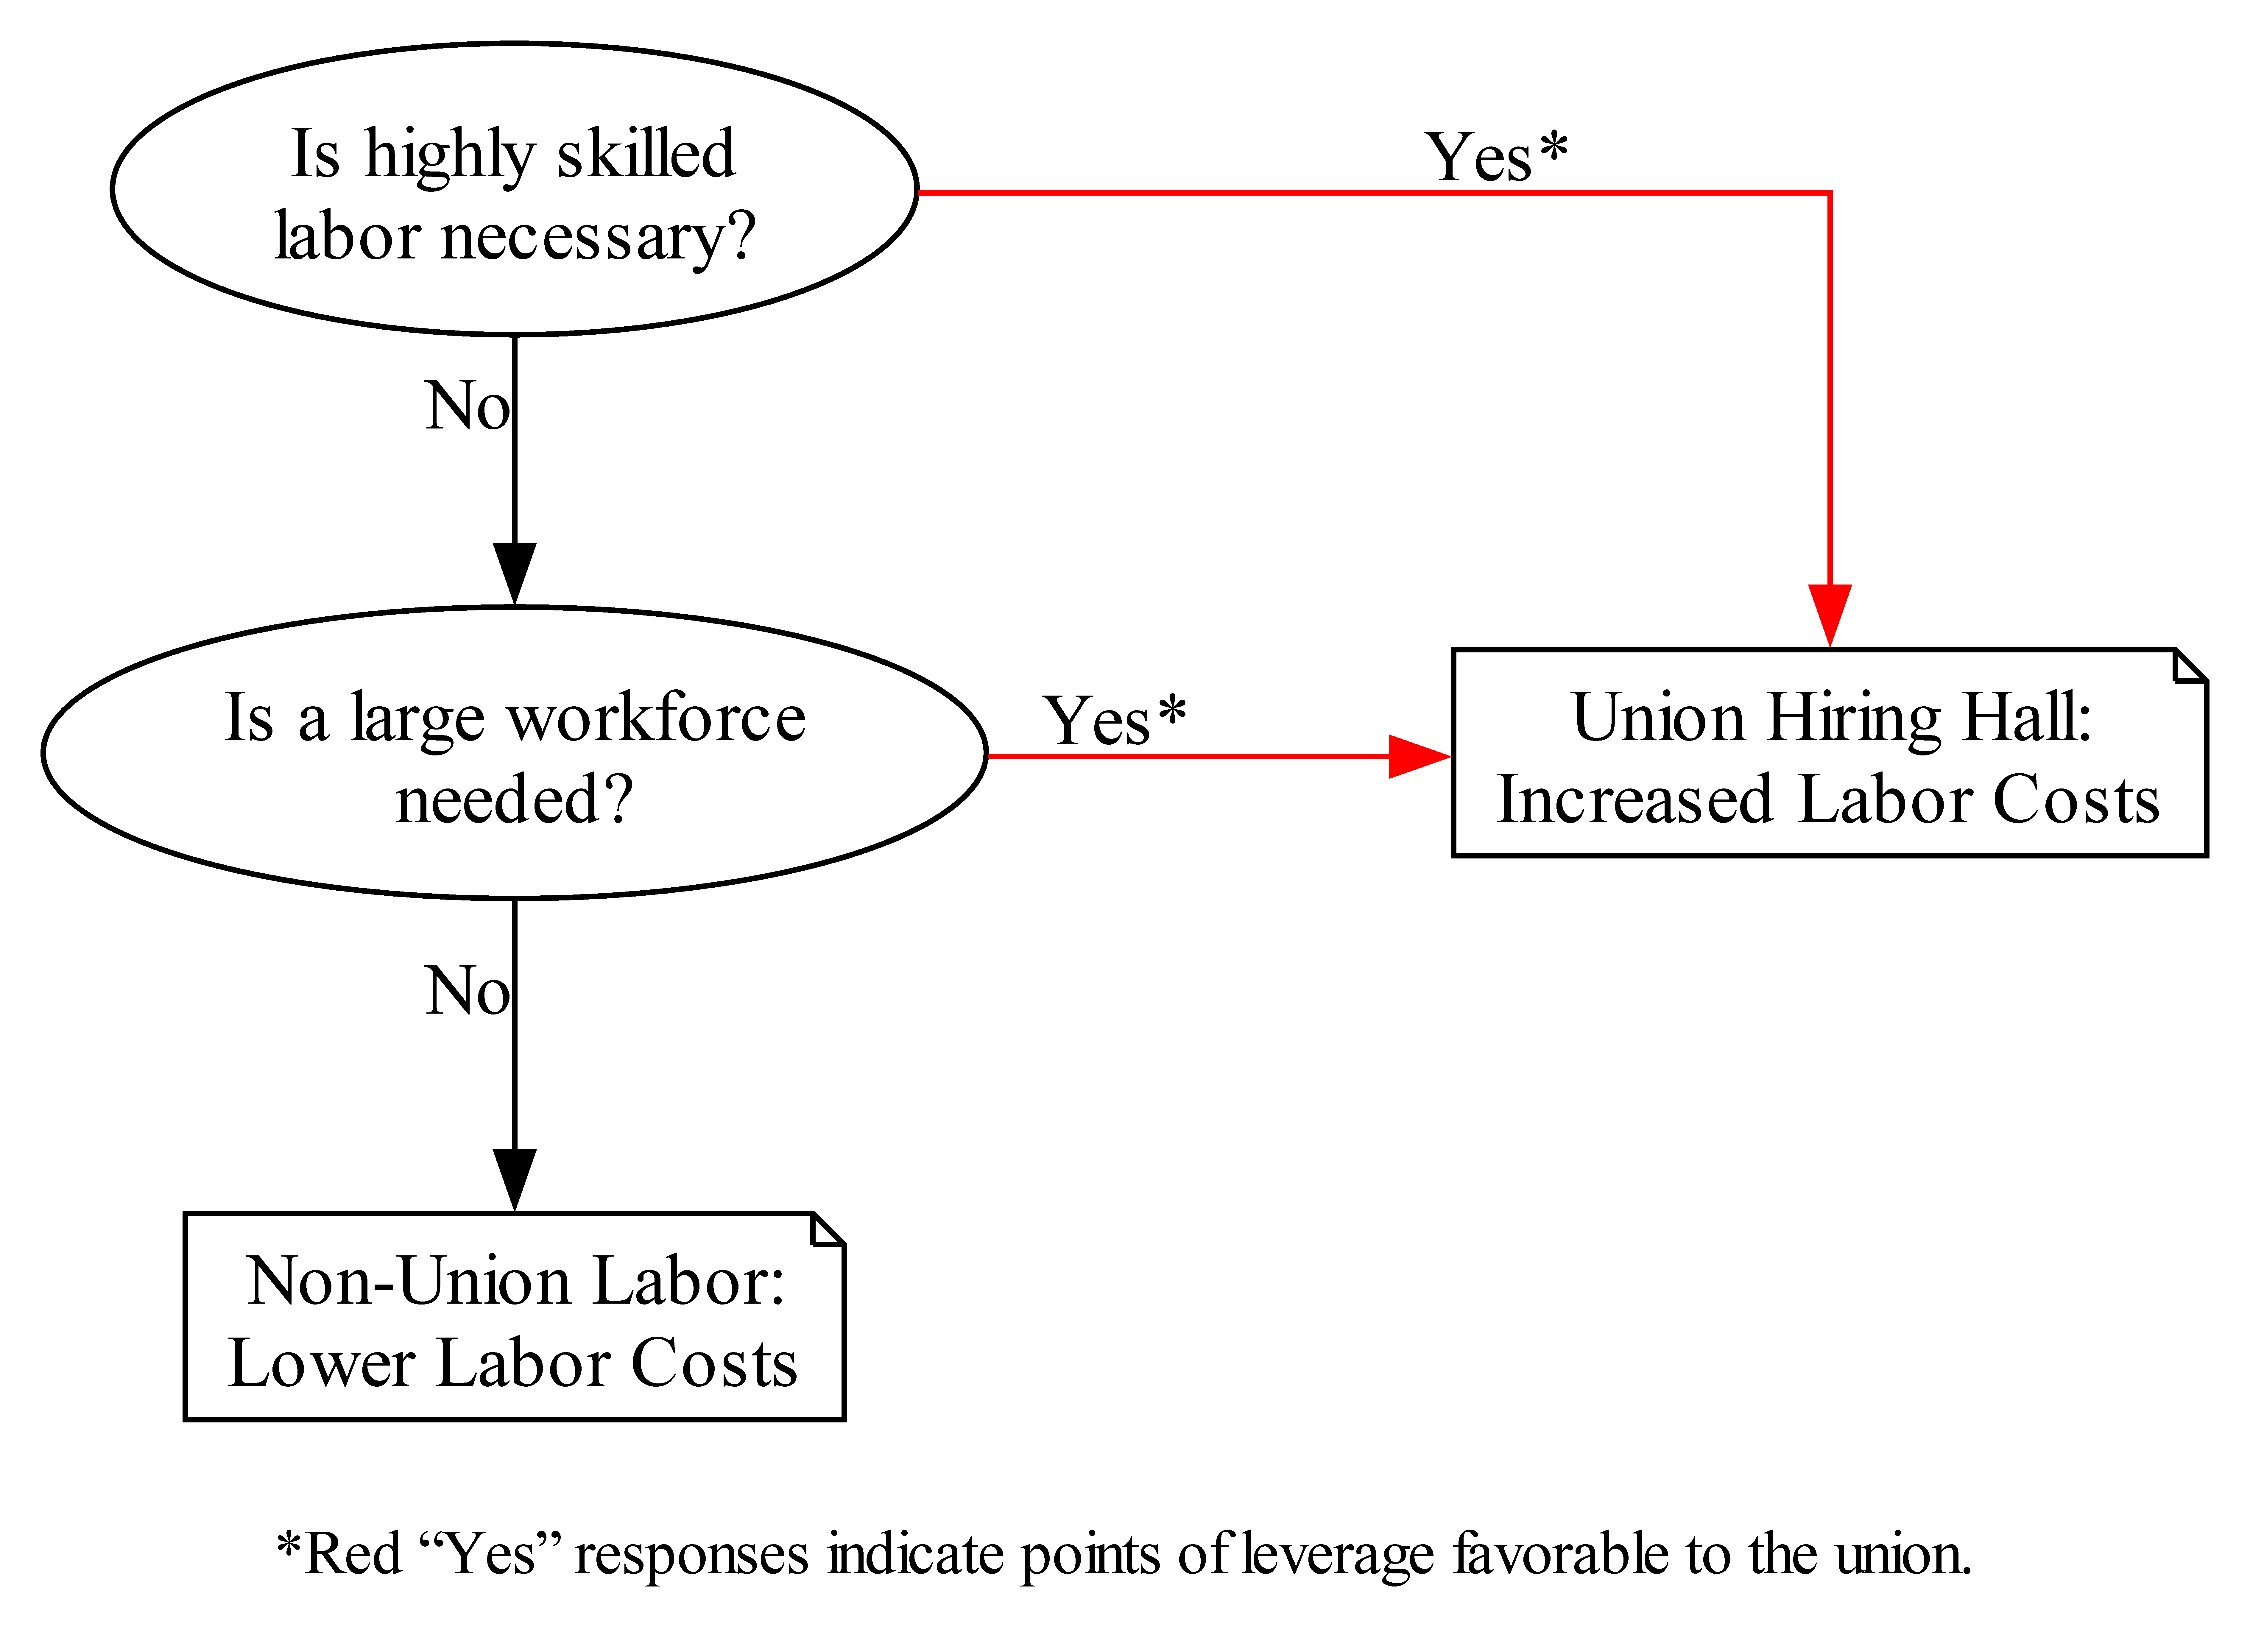
\includegraphics[width=\imageWidth]{images/union_power_red}
  \captionsetup{justification=centering, singlelinecheck=false, margin=2cm} 
  \caption[Union Leverage and Power]{Since negotitations between construction unions and employers are voluntary, construction unions typically have more leverage where the employer requires a more skilled workforce or where the job is large and requires many employees.}
  \label{fig:union_power_red}
\end{figure}

\subsubsection{The Hiring Hall}

The hiring hall is a central component of the prehire contract arrangement; they go hand-in-hand. Its development is largely due to the particularly contingent nature of construction work:

\begin{quote}
Many construction industry employers hire employees, as the need arises, to work on a particular project and to be laid off when their services are no longer required. Most construction workers are organized into union hiring halls. A hiring hall, or work referral system, is an arrangement under which a union that "has control of or access to a particular labor pool agrees to supply workers to an employer upon request." When an employer in the construction industry needs skilled workers for a project, he often seeks such workers from the union hiring hall. Historically, the practice in the construction industry was for the employer to sign an agreement with the hiring hall union which set the terms and conditions of employment for workers \textit{not yet hired}. These contracts, known as pre-hire agreements, often contemplated a tenure of years, spanning several projects. Rather than having to renegotiate the terms and conditions of employment on each new project, the employer was assured a ready supply of skilled workers and predictable labor costs upon which to base his bids on projects subcontracted by a general contractor. Furthermore, the construction worker had the benefit of a central clearinghouse for employment opportunities. (\cite[1014–1015]{murphyPreHireAgreementsSection1982}; emphasis added)
\end{quote}

Construction unions had been operating in this way for many years prior to the exemption to majority status requirements that were carved out for construction unions in Section 8(f) as part of the Landrum-Griffin Labor-Management Reporting and Disclosure Act (LMRDA) of 1959. In fact, before its enactment, the prehire agreement constituted a violation of the law which had, up until that point, required the union to show that the majority of employees wanted representation from that particular union. Murphy explains how the particularities of the construction industry made other modes of union organizing and operation difficult:

\begin{quote}
The periods of employment in the construction industry are often so short, however, that it is impracticable to complete the process of certifying a collective bargaining representative before a project ends and the employees are laid off. Furthermore, if an employer recognizes a union as bargaining representative of his employees, but the union is not in fact supported by a majority of his employees, the employer has committed the unfair labor practice of illegally assisting a union in violation of section 8(a)(1) of the National Labor Relations Act (NLRA). Pre-hire agreements, therefore, technically constituted illegal assistance of a union by the employer because agreements were signed prior to the union attaining majority status, indeed before the employer had even hired any employees. (\citeyear[1016-1017]{murphyPreHireAgreementsSection1982})
\end{quote}

To which the NLRB’s response was to ignore the violation until the 1959 passage of the LMRDA:

\begin{quote}
The General Counsel for the Board recognized the need of the construction industry to have a skilled work force available for quick referral and adopted a policy of not issuing complaints against construction employers and unions entering into pre-hire agreements. Finally in 1959, Congress legitimized pre-hire agreements by enacting section 8(f) of the NLRA. (Murphy p. 1017)
\end{quote}

In Senate debate, many senators acknowledged that this way of organizing in the construction trades was long-standing and informally ignored by the Board and courts. For example, Senator Javits recognized that the Taft-Hartley law, which LMRDA was to amend, was not being applied at the time:

\begin{quote}
We cannot apply the Taft-Hartley law to the building and construction field. We all know the law is not being applied in that field, and we might as well recognize the fact in the law. This is an essential amendment, and the sooner we adopt it the better. (105 Congressional Record, 86th Congress, 1st Session (1959), p. 6395) 
\end{quote}

Nor was this a regulation "imposed from above" to stifle trade unionism the way that Taft-Hartley was a dozen years earlier. Senator Dirksen acknowledged that labor wanted this amendment and had even approached senators about it in the years before LMRDA’s passage:

\begin{quote}
I remember that 2 years ago, when Mr. Richard Gray, the head of the Carpenters Union, came to the reception room with the General Counsel of the Department of Labor, they presented to us a proposal on the so-called prehiring agreements in the construction industry. They said, "This is what we want." (105 Congressional Record, 86th Congress, 1st Session (1959), p. 6414)
\end{quote}

%A few years earlier in 1956, the United Brotherhood of Carpenters’ magazine, the Carpenter, the official publication of the union spoke favorably of the bill because it would allow contractors and building trades unions [to] carry on contractual relationships in the way they have for over 50 years (https://archive.org/details/carpenter76unit/page/n5/mode/2up?view=theater pp. 7-8)

\begin{figure}[ht]
  \centering
  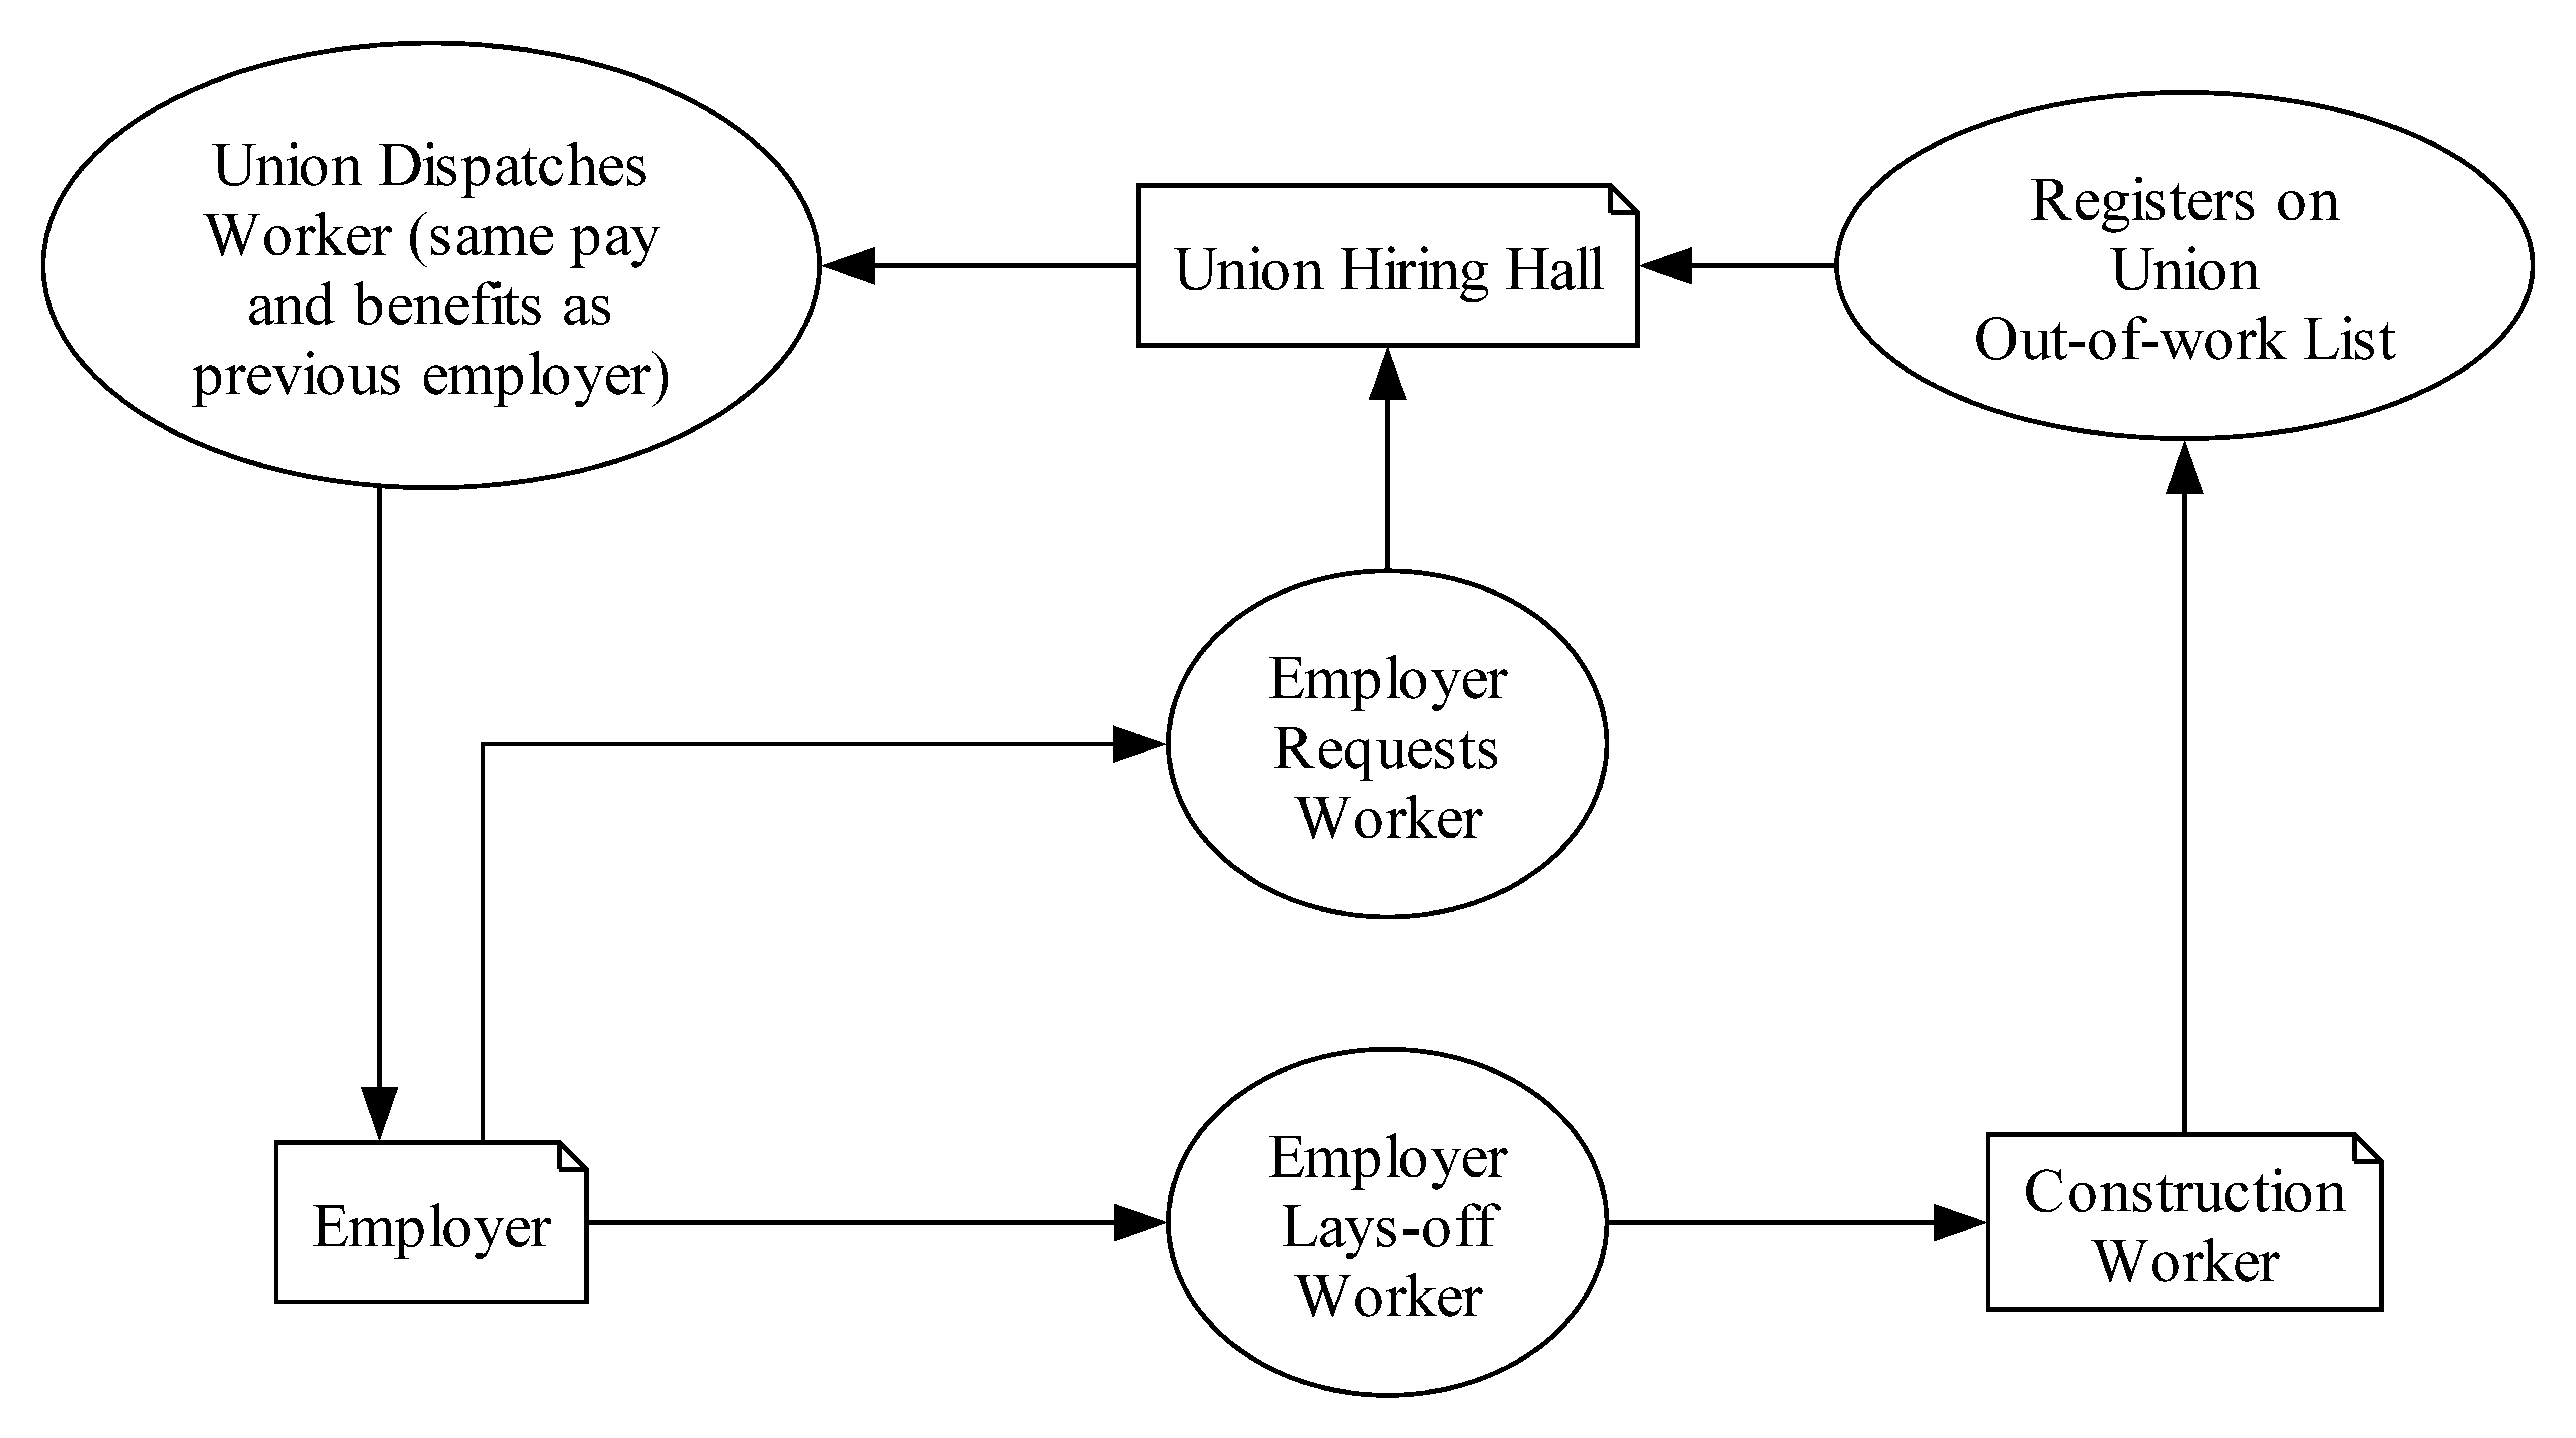
\includegraphics[width=\imageWidth]{images/hiring_hall}
  \captionsetup{justification=centering, singlelinecheck=false, margin=2cm} 
  \caption[Union Hiring Hall]{Construction unions usually maintain a hiring hall. When employers require more workers for their projects, they contact the hiring hall to request workers to be dispatched to the job site.}
  \label{fig:hiring_hall}
\end{figure}

\section{THE CASES} \

Cases that share similar features with the building and construction trades were selected for comparison: the Oil Chemical and Atomic Workers (now Steelworkers), a union that has many members working in the petrochemical industry, and the Machinists (IAM), a craft union that does not organize workers the way that the building and construction unions do. Also, an intra-building trades union comparison is made between the general building trades orientation and those building trades unions who have chosen to conduct NLRB elections in the same way that non-construction unions do.

The United Association of Plumbers and Pipe Fitters (UA) Local 189 in Columbus, Ohio was chosen because of the UA's large amount of pipeline and petrochemical refinary work. Richard Schneirov's \textit{Pride and Solidarity} was utilized to provide historical background on Local 189. Though it focuses specifically on Columbus, it is situated in the broder craft union currents of the time.

\subsection{The United Association of Plumbers and Pipe Fitters (UA) Local 189} \

In his masterful study of the United Association of Plumbers and Pipe Fitters Local 189 in Colombus, Ohio, Richard Schneirov (\citeyear{schneirovPrideSolidarityHistory1993}) details the uniqueness of construction unionism. The formation of the United Association of Plumbers and Pipe Fitters began in the late 1880s, Before then, plumbers and pipe fitters were largely unorganized; to the extent that they did form unions, the organizations were usually temporary, to meet a specific need at a particular time and were hyper-local and fragmented, without any international (a term that, in the context of US and Canadian unions, means a national organization) to push for the interests of plumbers and pipe fitters across the nation (p. 58). The first boon for the pipe tradesmen was not an organizing campaign undertaken by the union but the American Federation of Labor’s eight-hour-day movement (\citeyear[11, 43-45]{schneirovPrideSolidarityHistory1993}). Many pipe tradesmen in the late 1880s and early 1890s worked upwards of ten hours a day, sometimes up to fourteen hours per day. This movement was "of absolutely crucial importance. Hitherto, they had only been able to mobilize large groups of workers for short periods of time" (pp. 43-45). It also broadened solidarities, appealing to workers of "all natalities, races, trades, industries, skills levels, and genders" (p. 43). Indeed, though the eight-hour-day movement was largely associated with unionism, which provoked strong resistance from employers, it even appealed to non-union workers (p. 45). From that perspective, it was also able to "cement union sentiment and loyalty among large numbers of nonunion workers" (p. 45). And in contradistinction to earlier union efforts, this brought unions together across the nation, culminating in a nation-wide eight-hour-day strike on May 1, 1886. However, three days later the movement suffered a major setback when anarchists bombed the Haymarket Square in Chicago, killing seven police officers (p. 45).

However, the eight-hour movement’s efforts proved to be more durable, and on November 15, 1889, it gave rise to the formation of the first union of journeymen plumbers and pipe fitters Local 5180 in Columbus (p. 45). In 1890, Columbus streetcar workers continued to push for shorter workdays. They demanded a reduction from ten to nine work hours per day. In this context, the plumbers and pipe fitters were well positioned to exact concessions from the master plumbers because of fears that the latter could not defeat the former (pp. 45-46). The master plumbers agreed to a reduction in work hours without a loss in pay. However, the Local was inexperienced in negotiations with the master plumbers, and they were willing to make their own concessions to the employers that would allow the latter to severely restrict the time when overtime pay would start (pp. 46-47). The union sought the advice of the AFL founder Samuel Gompers, who disabused the local union from making concessions (p. 46-47). The two sides eventually reached a written agreement, the first of its kind in the trade. 

This encouraged the formation of the city’s first Building Trades Council (BTC). Despite earlier challenges in uniting the trades, the Council brought all crafts together: bricklayers, lathers, painters, carpenters, tinners, and plumbers and pipe fitters, under the banner popularized by the Knights of Labor: "An injury to one is the concern of all" (p. 47). And notwithstanding the master plumber’s earlier concessions, this inter-union trade solidarity set the stage for even more militancy. The BTC opted, in the words of the Columbus Dispatch, "for ‘radical measures’ at the opening of the ensuing building season" (p. 47). They demanded that union workers, no matter the craft or trade, perform the work on every union job site (p. 47). If their demand was not honored, the BTC threatened to not "touch any job" where non-union workers were present. Simply put, this meant that if one craft were union on a job site, that union workers on the site would refuse to work there unless every other craft were also unionized.

But by 1892 the union had pivoted to issues concerning the integrity of the craft. The union framed this in the language of public health, as the Columbus Trades and Labor Assembly contended that "nearly all the houses that are built for renting purposes are fitted with bad plumbing causing disease and death" (pp. 47-48). In response to these issues, the Assembly pushed for the city to adopt building codes and endorsed a union plumber for city inspector (p. 48). Consistent with this, the union began to place greater emphasis on the development of an apprenticeship program; the union asked the master plumbers for another raise and the establishment of an apprenticeship program "governing the number and conduct of apprentices" (p.48). The master plumbers refused, and the union went on strike. The master plumbers brought in strikebreakers, and the union eventually lost.

But the plumbers and pipe fitters union had not entirely abandoned broader solidarities. They continued to be involved in the BTC and in the Trades and Labor Assembly in an effort to "advanc[e] labor’s political strength" (p. 50). One leader epitomized the class-based orientation of the era: Louis Bauman. Bauman was the vice president of the Trades and Labor Assembly in 1893, and, beginning in 1894, he also served as the president of Local 57 of the plumbers and pipe fitters. He "was a Labor-Populist, aligned with radical farmers in the Farmers’ Alliances and the national People’s party and with the union men who felt that something should be done to change an economic system in which workingmen were impoverished while Wall Street banks and national corporations dominated the government" (p. 50). The Columbus Trades and Labor Assembly’s 1894 constitution exemplified its radical principles:

\begin{quote}
It is self-evident that, as the power of capital combines and increases, the political freedom of the masses becomes more and more a delusive force. There can be no harmony between capital and labor under the present industrial system for the simple reason that capital, in its modem character, consists very largely of rent, interest, and profits, extorted from the producers, who possess neither the land nor the means of production, and are therefore compelled to sell their labor and brains or both to the possessor of the land and means of production at such prices as an uncertain and speculative market may allow. Organization of Trades and Labor Unions is one of the most effective means to check the evil outgrowths of the prevailing system. (p. 50)
\end{quote}

However, the radicalism of the nascent pipe trades union was fraught with contradictions. In the early 1890s, the union had moved to exclusive agreements. These agreements offered lucrative benefits to entice the master plumbers into a contract. It not only limited the smaller firms’ ability to compete with the master plumbers by requiring union plumbers and fitters to work exclusively for the master plumbers, but it also precluded workers from "handl[ing] any materials not purchased by their immediate employers" (p. 54). In exchange the master plumbers agreed to allow "the union to set standard rates for the trade," and "offered local unions benefits that they had great difficulty winning otherwise: a closed shop, the eight-hour day, and stable or increased wages" (p. 54). At the same time, these agreements undercut the union’s bargaining power and leverage and, in many ways, the interests of union members. In particular, it limited employment opportunities for union members because non-signatory contractors could not employ union members even when paying union wages and adhering to union rules; this also hindered "the freedom of action of the unions" (p. 54). Eventually, the contractors’ demands undercut the union’s power so much that the union abandoned the practice of exclusive agreements in 1899 (p. 54-55).

Ironically, the abandonment of these exclusive agreements did not trigger union militancy or radicalism, and by the early 1900s, the union had all but entirely abandoned any commitment to improving working conditions; significantly, they also abandoned the broader labor solidarities that had defined the earlier period. If one word were to characterize this period, it would be "stability." Many unions in the late 1800s were temporary organizations. Indeed, as Schneirov observed, the telephone book and the UA’s official journal suddenly ceased to list Columbus UA Local 57 in 1898; it had completely disappeared without any historical record of what precipitated its collapse (p. 51). To achieve stability, American craft unions, following in the tradition spearheaded by the British craft unions, rose their union dues and implemented a quasi-welfare state. At the time, there was no "social safety net" provided by government; no unemployment benefits; no workers compensation; no social security benefits; and no Medicare or Medicaid. 

With increased dues, unions were able to finance these benefits and, consequently, keep construction workers in the union much longer than they had previously (p.59). The Columbus plumbers and pipe fitters union could also afford to hire professional staff and leadership for the first time. The union hired full-time business agents, who served as "walking delegates," policing the job sites for contract violations and craft jurisdictional violations by the employers (p. 60). He also was an organizer, enrolling new members, and "pulling a job" if he could not resolve a workplace dispute through negotiation (p. 60). And though most employers did not utilize it, in November 1907, the union established a hiring hall as an institution that would later become a staple of construction unionism; the hiring hall required laid-off members to provide the business agent their names so that he could register them on the list of unemployed members and dispatch them, beginning with the first member laid off to the member most recently laid off, at the employers request (pp. 60-61). And finally, this era ushered in intra-craft solidarity: plumbers and fitters for the first time began to see themselves not as individuals trying to "better themselves in the marketplace, hoping not to ultimately become independent masters, but as workers with shared interests with other plumbers and fitters (p. 61). These developments made the union into a more durable institution.

\subsubsection{A contemporary view}

Schneirov contends that the plumbers and pipefitters have had to balance between two sometimes contradictory identities. One is that they are workers with a set of common class interests with other workers in a labor movement built around solidarity for "union brothers and sisters." But from another perspective, they are part of a craft community that values craftsmanship and that takes pride in its work, a value that they share with their employer (Schneirov 1993:3–4) . A construction journeyworker is distinct in this regard from other blue-collar workers, such as factory workers on an assembly line, who do a repetitive task that can be easily taught (Schneirov 1993:5). Before one can become a journeyworker, one must complete an apprenticeship, which requires learning how to apply general plumbing and pipe fitting installation techniques, principles, and codes to specific circumstances. This requires a rigorous training program to prepare apprentices for their career. Because of this, these workers have gained prestige and a sort-of elite status that many other blue-collar workers could only dream of.

At the same time this elite status and craft pride also comes with a much higher degree of collaboration and much closer relationship with the boss. In fact, in Local 189, as is the case with many other plumber locals across the country, there can be a blurred line between employer and union member, and some union collective bargaining agreements even allow for contractors, that is, the owners of the enterprises, to work on projects alongside union employees (Schneirov 1993:5). This is also the case with UA Local 342 in the San Francisco Bay Area. Local 342 allows employers no more than one owner of the company to "work with the tools," so long as " the Individual Employer has not more than two (2) journeymen and one (1) apprentice dispatched" (Local 342 MLA). Many of these employers who also work "work with the tools" are members of the union. For example, Brown 3 Plumbing in Oakland, California is owned by William Brown, a Local 342 member who also works on many of his company’s projects (website). LJ Kruse Company in Berkeley, California similarly has members of the Kruse family who also work on the job site. Will Kruse has both completed the 5-year apprenticeship and serves as the company’s Vice President and Service Manager. He can be seen on the company’s website donning construction gear with a dirty high-visibility vest and jeans on a job site with a pile of steel framing in the background. And at Local 159 in Martinez, California, Brian Lescure, part of the Lescure family that owns Lescure Company, is both the Union’s Apprenticeship Coordinator and elected to the Union’s Examining Board (Lescure n.d.; Local 159 n.d.).

This has blurred line can give workers a sense, much more so than in other industries, that both employer and employee are on the same "team." And unlike an industry such as manufacturing, where large amounts of capital are necessary to start a business, starting a plumbing business is not unrealizable. One survey even found that half of a large plumbers local "had thought of entering business on their own at one time or another, though most had not done so" (Schneirov 1993:5). Put straightforwardly, this means that half of the local union’s workers, that is, sellers of labor power, also imagine a future as buyers of that same labor power. Schneirov contends that this blurring of the lines and class collaborative dynamic creates a "craft community," where employers and workers share a common background that "breed an ethic of cooperation among individuals based on mutual respect for craft knowledge, skill, and ingenuity" (1993:6). And "Even those union members who have never considered contracting have often bid independently on small jobs and are familiar with the psychology of being an entrepreneur" (Schneirov 1993:5,6). 

% Add a section here about the DAPL and how the building trades have responded.

\subsection{The Oil Chemical and Atomic Workers/United Steelworkers (USW)} \

The United Steel Workers (USW) and the Building Trades both have substantial work in the petrochemical industry. The Oil Chemical and Atomic Workers Union (OCAW) represented workers in the petrochemical industry for much of the 20th Century, but by the 1980s, membership numbers began to decline significantly. They merged with several other unions to form the Paper, Allied-Industrial, Chemical and Energy Workers International Union (PACE) in 1999. However, that merger only lasted 6 years, and they merged with the United Steel Workers in 2005.

The Oil Chemical and Atomic Workers were much more radical than other unions, and as Mark Dudzic, a former leader and retired member once described it, "The oil industry never really accepted the union as a junior partner. The union was never able to win the union shop and all the other accoutrements of class peace. As a result, the culture of militancy was deeply embedded in the union" (Leopold 2007). Though the OCAW is now dissolved, and has gone through two mergers, it is worth tracing the history to the present day to analyze if their radical history has had any lasting effect, and if the lack of class peace persists.

Unlike the Building Trades, the USW is currently a supporter of the Labor for Single Payer Health Care campaign, which is a broad social-wage political effort. From that perspective, the USW is not just focusing singularly on their members’ interests but is instead committed to broader political struggle. Strikingly, the USW even supports a transition from dirty-energy to clean-energy jobs. This is significant for a union that has many workers in the petrochemical industry. Such a transition would end their employment at oil refineries and require a new, more challenging struggle to establish a union foothold in new clean-energy sectors, sectors that have been highly resistant to unionization. Nevertheless, the USW has adopted a broader, more long-term vision, one much more solidaristic with other environmental activist groups than the Building Trades have.

\subsection{OCAW and Tony Mazzochi}

Les Leopald, in \textit{The Man Who Hated Work but Loved Labor}, recounts the story of Tony Mazzocchi, former long-time Oil Chemical and Atomic Worker official and organizer. In looking at the history of this union with Tony as the leading protagonist Leopald highlights the social unionism that the former helped craft in the postwar period in New York (p. 16).

Tony started his employment at Helena Rubinstein Incorporated on May 1, 1950. Union leaders of the left-leaning District 65 had recruited Tony to raid an anti-communist CIO union. At the time, District 65 was the largest left-leaning union in New York City. It had disaffiliated with the Retail, Wholesale, and Department Store Union (RWDSU) in August 1948 after the national union had ordered the District to comply with the Taft-Hartley Act, an act passed in 1947 that substantially gutted the Wagner Act  and imposed onerous burdens and restrictions on labor unions, severely curtailing their power, so much so that it was commonly denounced by labor as the "Slave Labor Bill" (Figure \ref{fig:slave_labor_bill}). The District 65 leaders were Communist Party members or sympathizers and wanted Tony to obtain employment at a unionized New York City cosmetics plant, Helena Rubinstein Incorporated, as a "colonizer." His role would be to organize a progressive cadre within the rank-and-file of the Gas, Coke, and Chemical Workers local union, which was present at the plant (p. 71). They wanted him to work his way up through the leadership ranks and bring the local into the left-leaning District 65. Tony got hired on in May 1950; and through this effort Mazzocchi got his start as a union organizer.

\begin{figure}[ht]
  \centering
  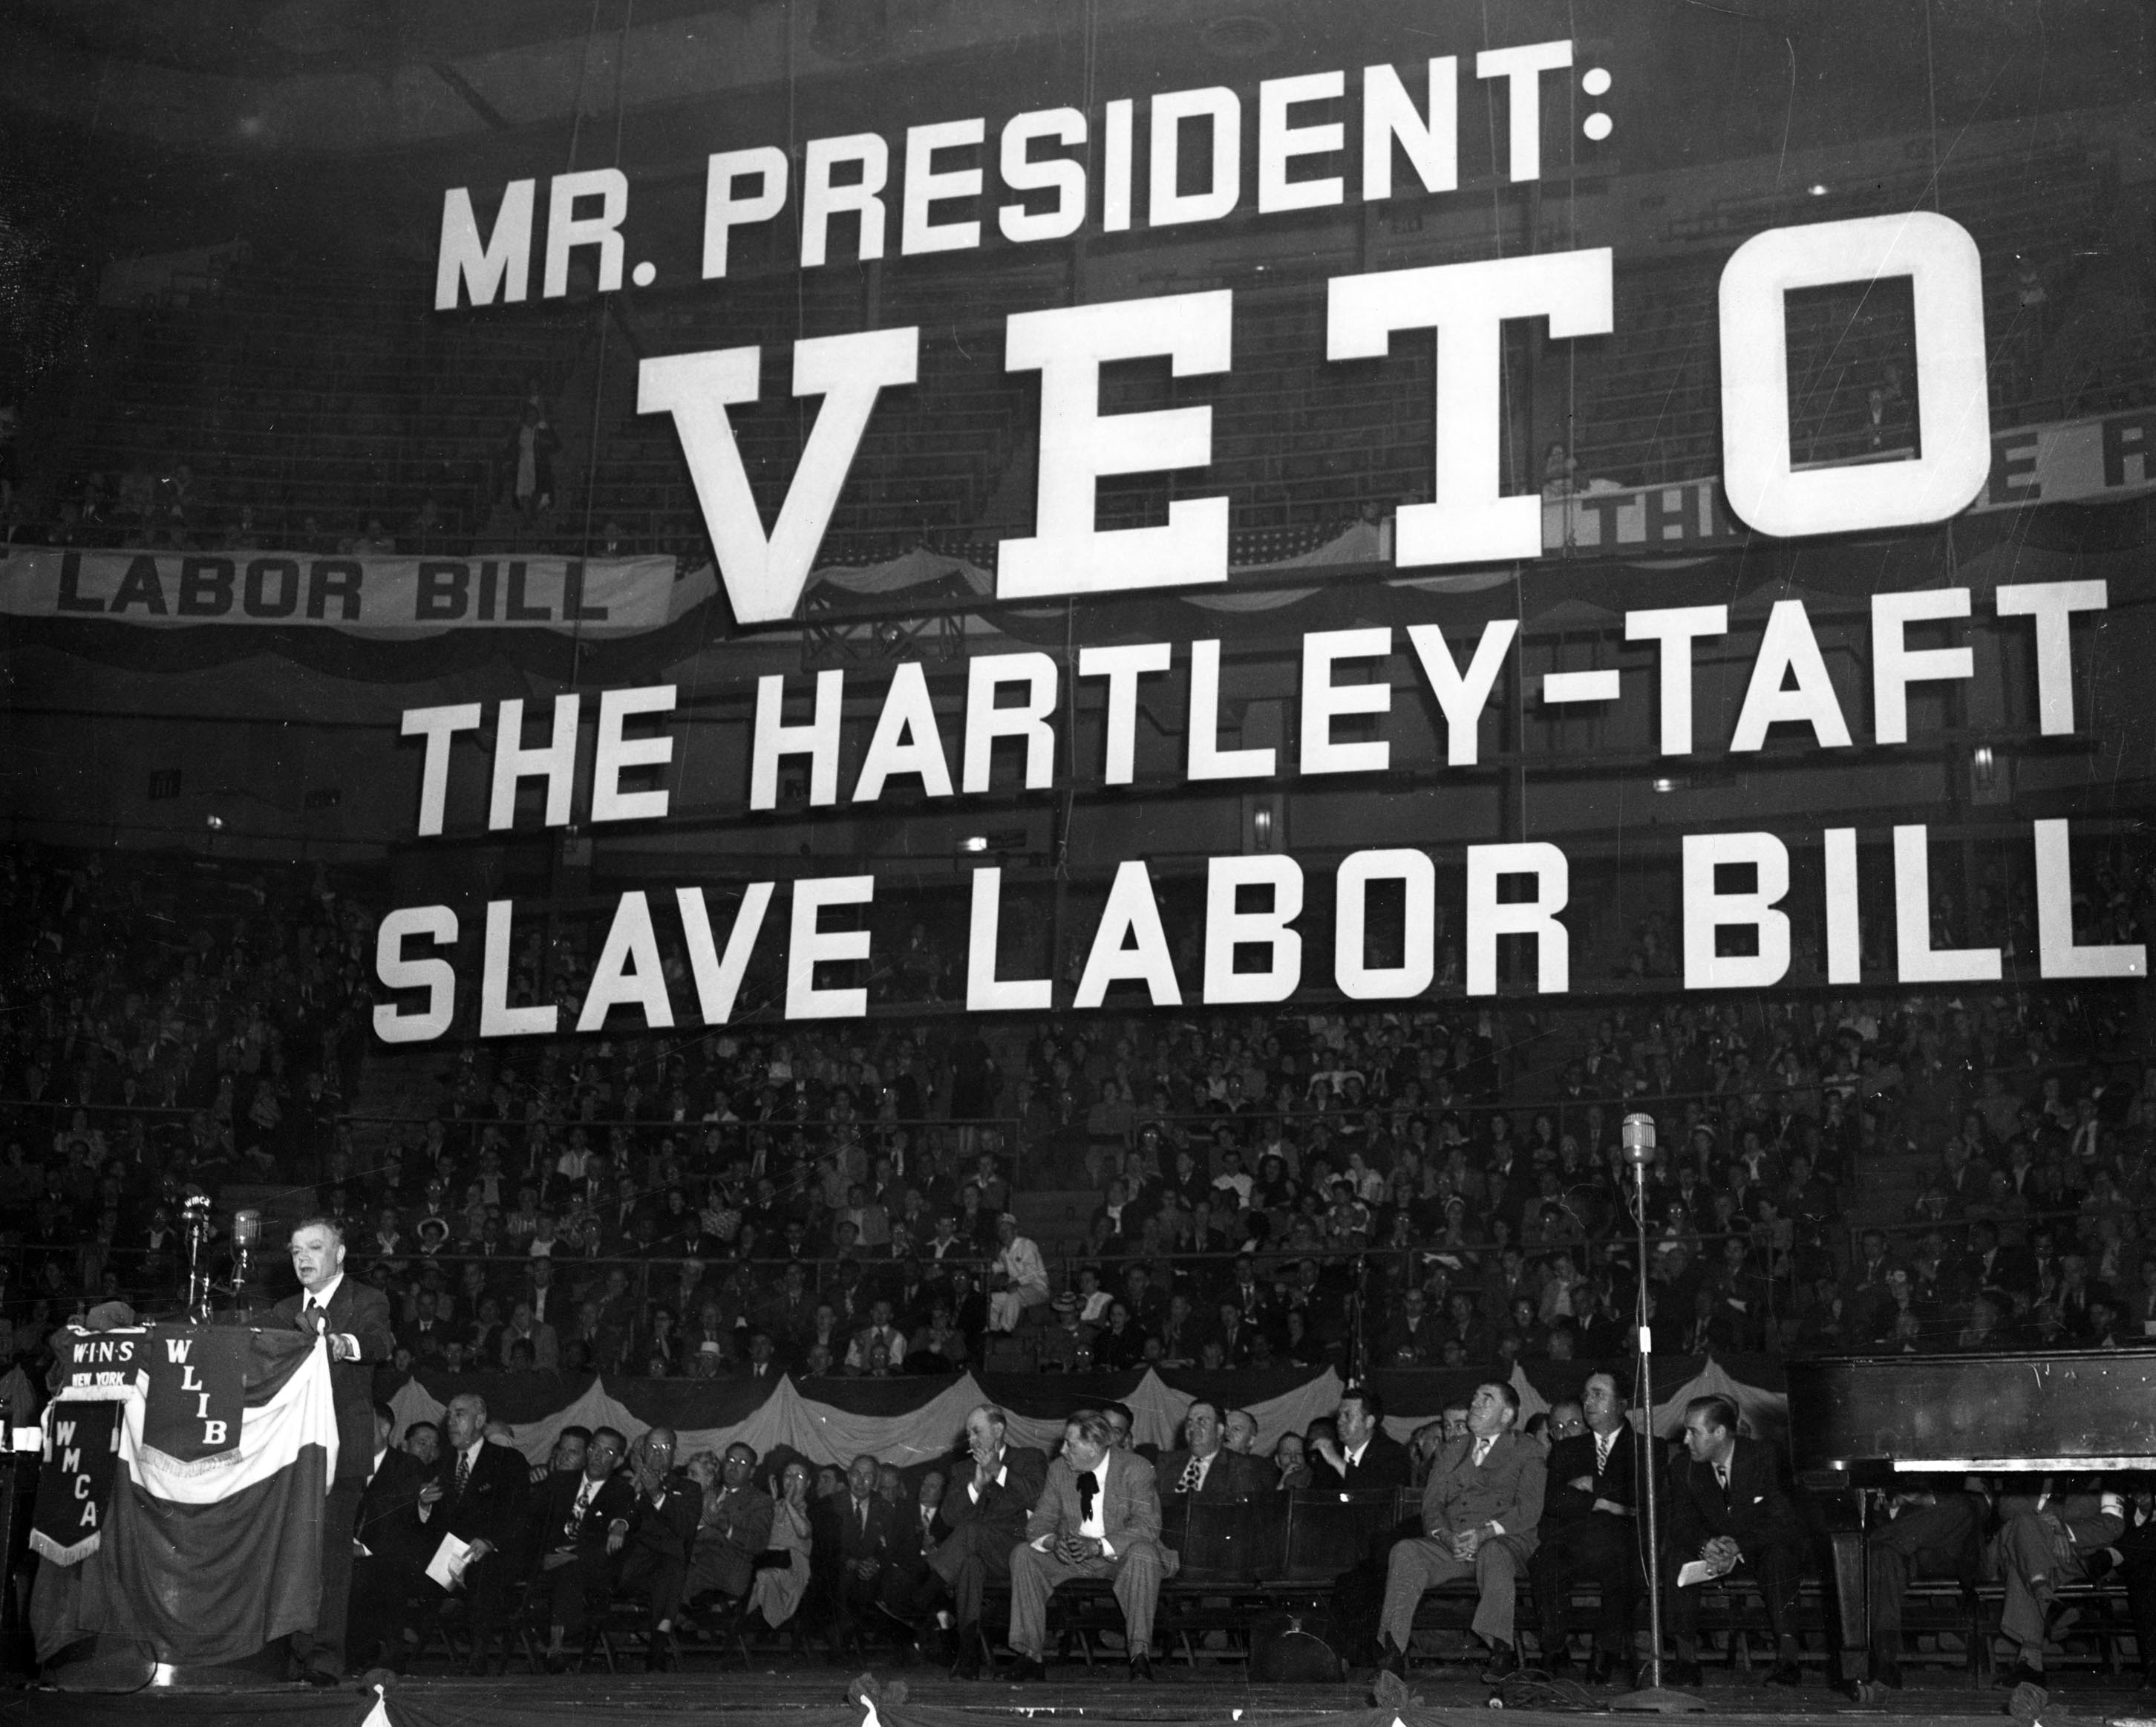
\includegraphics[width=\imageWidth]{images/slave_labor_bill}
  \captionsetup{justification=centering, singlelinecheck=false, margin=2cm} 
  \caption[Anti-Hartley-Taft Rally]{David Dubinsky of the International Ladies Garment Workers Union (ILGWU) gives a speech against the Hartley-Taft bill, with Luigi Antonini in the audience, May 4, 1947.\\ (Source: \href{https://www.investopedia.com/thmb/VcswppMRTl8IqMbgLRqdigfIGvs=/1500x0/filters:no_upscale():max_bytes(150000):strip_icc()/5278798677_0429e6aa05_k-7b6b81bdbbe44cdb929c08c7da9f8d29.jpg}{Investopedia.com}) \nocite{investopediaMrPresidentVeto}}
  \label{fig:slave_labor_bill}
\end{figure}

These years preceded the formation of the Oil Chemical and Atomic Workers (OCAW). It wouldn’t be until March 4, 1955, when the Gas, Coke, and Chemical Workers (UGCCWA) merged with the Oil Workers International Union (OWIU) to form the OCAW (OCAW 1960, p. 48). This was also the year when the AFL and CIO also merged, forming the present-day AFL-CIO.

\subsubsection{The Oil Workers International Union}

Oil workers’ first breakthrough in terms of organizing occurred during World War I in Texas and California. The Congress of Industrial Organizations (CIO) had not yet formed, so a charter in the American Federation of Labor (AFL) was granted to several local unions; once several of these locals were chartered, they successfully petitioned the AFL for a charter as the Oil Field, Gas Well and Refinery Workers of America in 1918 (OCAW 1960, p. 48). After some initial success, the union’s membership began to decline to merely 350 by 1933 because of union busting aided by the federal government, but the passage of the National Labor Relations Act in 1935 gave the union a new set of rights and tools to organize, which again gave the union a boost (p. 49). That same year, the president of the union worked with other labor leaders to establish the Committee for Industrial Organizations, though they still remained within the AFL ; but this did not last long and two years later the Committee broke with the AFL to form its own union federation (OCAW 1960, p. 49). During the same period, the union’s internal democracy considerably improved with the creation of the rank-and-file International Executive Council, and officers were not longer elected by the convention; instead they were elected by direct referendum (pp. 49-50).

\subsubsection{Gas, Coke, and Chemical Workers}

The Gas, Coke, and Chemical Workers Union started in the United Mine Workers of America (UMWA). The UMWA wanted to unite workers in industries that processed or used petroleum coke in the production of artificial gas (OCAW 1960, p. 50). The UMWA was in the AFL at the time, and the Federation was resistant to their organizing efforts. After the UMWA left the AFL, it formed District 50, which was focused on organizing the "gas, coke, and allied products" industries (OCAW 1960, pp. 50-51). However, soon John L. Lewis, who was president of the UMWA at the time, split with the CIO, pulling the Mine Workers out of the CIO. This did not sit well with the gas coke workers within District 50; they had developed loyalty to the CIO, and were now merely a division within the now independent District 50 (OCAW 1960, p. 51). Because of this, the various local unions of gas and coke workers sought their own national union, and in 1942 they were granted a charter from the CIO as the United Gas, Coke and Chemical Workers of America (p. 51). No longer a part of the independent District 50, they were back in the CIO.  But by 1955, they decided to merge with the Oil Workers to form the Oil Chemical and Atomic Workers.

In the years before Tony Mazzochi entered the union, anti-communism was in full force. The Gas-Coke local union Mazzocchi had joined had a close affiliation with the Communist Party. Several prominent leftist union leaders, such as Fred Hamilton and Charles Doyle were key to the union’s strength and survival. Not only had several leftist leaders had organized the Rubinstein plant that Mazzocchi worked in, but the founding convention of United Gas and Coke Workers was held near Doyle’s home area of Niagra Falls (Leopold 2007, p. 81). Unlike many of the craft unions of the time, which were practically all white and male, Gas-Coke was forthright in its opposition to discrimination. They were early adopters of anti-racist policies and practices. They passed resolutions condemning racist discrimination at their founding convention, and urged for the promotion of more women in union leadership. Suffice to say, that despite the reactionary tide, the union managed to forge a genuinely progressive agenda, especially in light of the context in which they were operating.

Anti-communism by and large had not infiltrated the union’s rank and file either. For example, in 1946, the union voted to "provide financial support for the CP-dominated United Electrical Workers during its difficult Phelps-Dodge strike (Leopold 2007, p. 84). Notwithstanding the strong CP presence within the union, it still counted many anti-communists amongst its ranks, though they managed to work together relatively peacefully until 1946 (Leopold 2007, p. 82). It was at that time the anti-communists began plotting to take over the union and push the communists out. They eventually purged Charles Doyle from the union by holding a convention in Canada. Doyle did not have legal immigration status in the US. The anti-communists tipped off the INS, so that when Doyle tried to reenter the US, he would be denied. This effectively ended his OCAW tenure. Jack Curran, an anti-communist rose to power within the OCAW.

Mazzocchi had connections with the CP through family and relatives, though Mazzocchi himself was not a member of the party. He was, however, politically active and looking for a job. At the same time the purged communists were looking for revenge and to take back the union from Curran and the anti-communists. Mazzocchi got his start in the union as part of this effort. In moderating the politics of the union, Curran had been ineffective at warding off the "power grabs" by management. Furthermore, the chief steward had let grievances pile up unaddressed (Leopold 2007, p. 90). This presented an opportunity for Mazzocchi to step in and slowly organize to win workers over to his vision of what the union ought to be. He started by addressing agitating around the inadequate handling of grievances at the Rubinstein plant where he worked and eventually ousted the conservative steward at the plant. Slowing he worked through the ranks of union leadership, getting elected to the local’s committee at the Gas-Coke District Council and speaking up about issues at the union meetings (Leopold 2007, p. 97-98). 

Over the years the union maintained itself as a progressive voice within the labor movement. Despite having so many members in industries that work with environmentally hazardous chemicals, the union developed a plan for what it called a Just Transition: an effort to advance a politics that both protected the environment from hazardous chemicals and emissions and the workers who would be affected the most by transitions away from those processes and usage of those chemicals. Indeed, in the 1990s, the union  spearheaded the effort to build the US Labor Party, a party independent of the Democrats and Republicans anchored in the trade unions. It also was instrumental in the creation of the Chemical Safety Board (CSB) after the explosion at the Phillips Chemical Plant in Pasadena, Texas killed 23 workers (author correspondence with Mark Dudzic). The OCAW was heavily supported and pushed for the passage of the Occupational Safety and Health Act, which created a federal agency to enforce occupational safety laws. The union was also a driving force in the passage of the Environmental Protection Agency.

Though the union maintained a progressive voice within the labor movement throughout the period, it continued to shed members throughout the 1980s and 1990s, largely to offshoring of production, automation, and deindustrialization (Dudzic 2024). For example, plants that used to require 10,000 workers to operate now can be run with as few as 600 or 700. Ironically, many of the stringent occupational and environmental health and safety laws that the union advocated for also made production more expensive in the US and possibly contributed to the union’s decline in membership via offshoring and globalization. According to Mark Dudzic, former OCAW official, the bosses were quite frank in conversing with the union about what was driving their decision to move production outside the US. For example, over the years the union had fought to improve safety at one of the plants where they had members. Approximately 120 workers at the plant were frequently exposed to very hazardous chemicals; the union finally convinced the employer to build a wastewater treatment plant and install enclosed production booths to mitigate the hazards. However, the company eventually decided to move production to India. The union tried to negotiate with them to no avail. The company had a  \textdollar 10 million annual wage bill, and environmental compliance costs of  \textdollar 15 million per year. In India environmental compliance costs were close to zero and wages much lower (Dudzic). According to Dudzic, the company would tell the union:

\begin{quote}
Our wage bill is \textdollar 10 million a year. Our environmental compliance is \textdollar 15 million a year. It's close to zero in India. So you could offer to work for free, and it still wouldn't be competitive with what we can do in India because of the environmental compliance. So, basically, they were offshoring not only our work but their ability to contaminate workers and communities. This plant had one of the highest rates of bladder cancer in the United States before we started organizing these protections and I'm sure the rates of bladder cancer wherever they moved to in India went up because of this company. (Dudzic 2024)
\end{quote}

In 1999, to "stop the bleeding," the OCAW merged with the Paper Workers Union to form Paper Allied Industrial Chemical and Energy Workers (PACE). Dudzic described this merger as disastrous:

\begin{quote}
The [Paper Workers had] opposite tradition in terms of internal governance was very top down, very closed; officers basically ran the show. They had these district directors who manipulated politics in the various districts, so it was very opposite of the OCAW. Some people in our Union felt that we could shake things up; they promised to allow for some more democratic structures in the new Union, but they quickly closed the doors on that after the merger. The hope was that the paper workers were … the structures of the industries were very similar, these large manufacturing facilities dominated by multinational corporations; the Paper Workers, like the Oil and Chemical workers, had a lot of people in the South and in rural areas. There was some sense that there could be some synergy there, but the leadership was backward, incompetent, and intent from the very beginning on purging any kind of militancy and progressive politics from the Union. (Dudzic 2024)
\end{quote}

The merger also threatened the Just Transition framework that the OCAW had pioneered:

\begin{quote}
Those guys didn't like it [Just Transition]. You know, we had this big fight about chlorine which is a key ingredient in the paper making process but there [are] other technological ways to make paper without using chlorine. And we, the Oil, Chemical Atomic Workers, had called for a ban on chlorine. And the Paper Workers sided with the industry and opposed that ban; that was one of the first fights we had after the merger, and we lost, and that was sort of the defeat of the worker-centered, just transition model as opposed to an industry supportive, "keep pumping the poisons out as long as you can" model. (Dudzic 2024)
\end{quote}

However, the merger was short-lived. In 2005, PACE was absorbed by the USW. Though the merger with the USW was also conducted in a top-down fashion (Dudzic), it had the effect of stabilizing the union, which had still been in a precarious position. The merger has effectively wiped out many of the earlier OCAW democratic rank-and-file decision-making processes and replaced them with more bureaucratic methods. For example, much of the negotiating activity is now carried out by "technicians," who closely study the economic trends in lieu of talking directly with the workers and "work[ing] from the bottom-up on…bargaining" (Dudzic 2024). At the same time, the OCAW culture around health and safety has survived. According to Dudzic, the USW had "always [been] a partner with the OCAW, from the days going back to the passage of the OSH Act in 1970" (Dudzic 2024). The USW’s Health and Safety Department is also named after Tony Mazzocchi. It is called the Tony Mazzocchi Center for Labor and Environmental Health.

This persists even in 2023. To wit, the Carson, California USW Local 675 has been supportive of several environmental initiatives and efforts. The Local, which it is important to note is an oil local, endorsed the Pollin Report released in 2021. The report charts a path away from dirty fuel sources to clean energy. More recently, in 2023, Norman Rogers, vice president of USW Local 675, was quoted in the Los Angeles Times as a supporter of a transition from fossil fuel to clean energy jobs. Several area local unions have launched a political coalition to lobby Sacramento to protect workers while the transition occurs. From that perspective, perhaps the most enduring feature that has survived from the OCAW days is the Just Transition framework.

%\subsection{The International Association of Machinists (IAM)} \

% The International Association of Machinists (IAM) and Building Trades both are unions in the craft union mold. Both were American Federation of Labor unions (before the 1955 merger), which was a labor federation largely rooted in craft unionism. Although perhaps not anchored as steadfastly to the expansion of social-wage policy and decommodified public goods as unions such as the National Nurses United and National Health Care Workers or even The Brotherhood of Maintenance of Way Employees, they have nonetheless given their official support toward the effort to establish single-payer healthcare in the United States, a policy that would eliminate private insurers and establish government-funded healthcare insurance that would cover all regardless of ones income or finances. This arguably is along the more "radical" edge of the US trade union movement, such as it is.

% What might cause a union that comes out of the craft union mold typically associated with very conservative politics and historically with racist, exclusionary policies and practices to support progressive social-wage policy that would cover not only its members, but the entire US population regardless of race, gender, ethnicity, or immigration status? One possible response is that it is ideological, that the Machinists have always been guided by a strong commitment to what Joe Burns has termed, "class struggle unionism." The issue with this is explanation is that it does not do much more than repeat the question by way of answer. That is to say, why are there these ideological differences? The other problem, which deserves further investigation, to be sure, is that that contention likely has little to no empirical support.

% The alternative hypothesis is that the material relations of production, forged in the context of particular bargining schemes, strategies, which often enough, are responses to pragmatic concerns and constraints, condition the way in which union workers and union leadership adopt a guiding ideology and orientation vis-a-vis the bosses. If the approach is successful, it continues into successive contracts and generations. This might be summed up with the common aphorism, "if it ain’t broke, don’t fix it." While this likely does not follow a strict determinism (for example, political pressures and conditions outside the union and organizers and agitators within the union advancing a different orientation vis-a-vis the boss exert their own forces), it nonetheless exerts force and places constraints on how union workers and leaders relate to the boss.

% With respect to the building trades in particular, they are responding to a particular set of historical circumstances that have placed constraints on their relationship with the employers. The most obvious one is the contingent nature of construction work. While in other industries and occupations, employees often work for the same company for their entire career (or at least for a duration spanning many years), construction workers are employed by a single employer anywhere from 1-2 weeks to 1-2 years.  This precariousness makes organizing the typical route (organizing the workers \textit{already employed)} impractical. Although the National Labor Relations Act (NLRA) often permits workers who were employed at the time the election was requested to vote, how effective of a strategy would it be to organize a workplace where it is in essence a revolving door in this fashion? From that perspective, "organizing the bosses" is a logical response to the question. But it also requires a strategy that is largely \textit{anti-conflictual}.

% On the other hand, the IAM, which is still anchored in the craft union orientation, does not have this "revolving door" problem. Much of their workforce is permanent, in fields such as manufacturing, on-site installation and service work.  Because of this difference in duration of employment, the IAM does not "organize the bosses" the way that the Building Trades does. This means that they can adopt a more confrontational strategy, one that does not seek to find common ground with the employer but one that compels the employer to respond to their demands and offer concessions. It is worth noting that this approach to organizing does not preclude class collaboration. Many of the unions that follow this route, for example the United Food and Commercial Workers, have notoriously opposed conflictual strategies. However, this approach at the very least leaves the opportunity for conflictual strategy vis-a-vis the boss open as a possibility, while the Building Trades approach largely precludes it because of their voluntary contracts. 

\subsection{Intra-Building Trades Cases} \

While the Building Trades largely "organizes the bosses"\footnote{A wonderfully apt description that I owe to Mark Dudzic, former OCAW official and long-time Labor for Single Payer Organizer.} rather than the workers already employed, there is still some variation in how they organize. A search of the National Labor Relations representation case petition database revealed that approximately 98 building trades unions have filed for a representation election in 2023. The results were obtained by removing company names that did not contain the words "construction," "constructors," "electrical," "plumbing," "mechanical," "builder," or "builders." If the certified representative matched the names of any of the Building Trades’ constituent unions, they were also added to the list. While this method did not filter out all non-Building Trades unions, it probably erroneously excluded some from the filtered list because it is nearly impossible to include every possible search term.



% This provides an interesting opportunity because building trades local unions that petition for a representation election are not following the usual organizing path. They are organizing the workers instead of the bosses. Interviewing the union organizers to understand what drove this choice of organizing over the usual building trades approach could produce interesting findings. Perhaps the union had to become creative in a difficult construction economy that threatened to reduce its membership. Possibly, workers in those shops reached out to the union because of workplace issues or low wages, and they sought unionization to improve their working conditions and pay. 

\newpage

\titleformat{\section}{\fontsize{12}{14}\bfseries\centering}{\thesection}{0.5em}{}
\printbibliography[title={Bibliography}, heading=bibintoc]

\end{document}
